\documentclass[11pt,a4paper,titlepage]{article}
\usepackage[czech]{babel}
\usepackage[T1]{fontenc}
\usepackage[utf8]{inputenc}
\usepackage[left=2cm,text={17cm,24cm},top=3cm]{geometry}
\usepackage{times}  %font
\usepackage[ruled,czech,linesnumbered,longend,noline]{algorithm2e}
\usepackage{algorithmic}
\usepackage{graphics}
\usepackage{picture}
\usepackage{lscape}
\usepackage{siunitx}

\begin{document}

\begin{titlepage}
                    %%%%%%%%%---TITLE PAGE---%%%%%%%%
\begin{center}
                      
{\Huge\textsc{ Vysoké učení technické v Brně }}\\
\bigskip
{\LARGE\textsc{ Fakulta informačních technologií }}\\
\bigskip
\vspace{\stretch{0.382}}
{\LARGE{Elektronika pro informační technologie}\\
\medskip
\textbf{\Huge Laboratoř č. 1}}
\vspace{\stretch{0.618}}

\end{center}
{\Large\today \hfill David Prokopec}
\end{titlepage}
    

\section{Zadání}

V laboratorním cvičení č. 1 bylo naším cílem získat základní schopnosti pro:

\begin{itemize}
  \item Zapojování obvodů dle schémat
  \item Měření elektrických hodnot pomocí multimetru
\end{itemize}

\noindent Následně jsme také experimentálně oveřili základní fyzikální zákony a související principy.

\subsection{První experiment}
Úkolem prvního experimentu bylo seznámit se s obsluhou multimetru. Připravili jsme si rezistor a následně jsme změřili jeho odpor. Poté jsme změřili napětí na rezistoru a proud protékající rezistorem.

\subsection{Druhý experiment}
Úkolem druhého experimentu bylo zjistit celkový odpor dvou odporů, které jsou zapojeny paralelně nebo sériově. Také jsme změřili napětí na rezistorech a proud protékající rezistory.
Schéma zapojení obou obvodů (obr. \ref{pic:obvod1} a obr. \ref{pic:obvod2})

\begin{figure}[ht]
\begin{center}
    \scalebox{0.4}{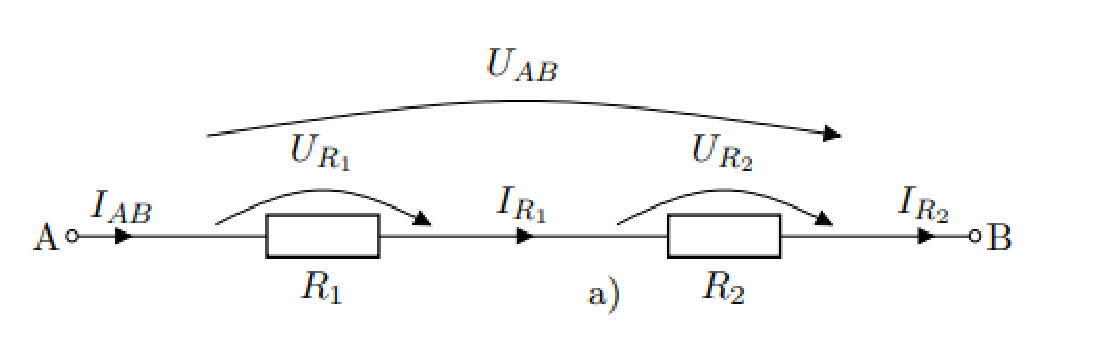
\includegraphics{obvod1.eps}}
    \caption{Schéma zapojení odporů sériově}
    \label{pic:obvod1}
\end{center}
\end{figure}

\begin{figure}[ht]
\begin{center}
    \scalebox{0.4}{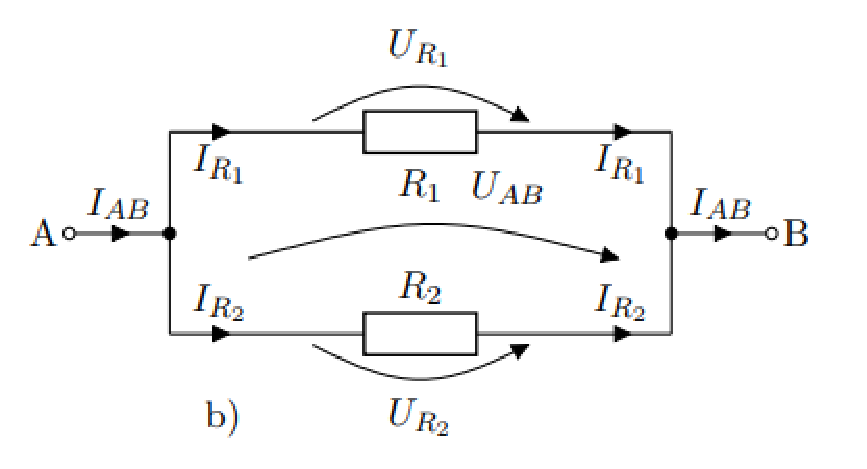
\includegraphics{obvod2.eps}}
    \caption{Schéma zapojení odporů paralelně}
    \label{pic:obvod2}
\end{center}
\end{figure}


\section{Teorie}

K měření základních elektrických hodnot lze použít multimetr. 

\begin{itemize}
  \item Pro měření napětí $U$ v obvodu se zapojíme paralelně s měřeným obvodem a multimetrem nastavíme na měření napětí.
  \item Pro měření proudu $I$ v obvodu se zapojíme do série s měřeným obvodem a multimetrem nastavíme na měření proudu. 
  \item Pro měření odporu $R$ se zapojíme do série s měřeným obvodem a multimetrem nastavíme na měření odporu.
\end{itemize}

\subsection{Ohmův zákon}

Pro ověření hodnot naších měření využijeme Ohmův zákon. Ten říká, že napětí $U$ na svorkách rezistoru je přímo úměrné proudu $I$ protékajícího rezistorem. Tato úměrnost je dána velikostí odporu $R$ rezistoru. 
\\ Tedy platí:

\begin{equation}
I=\frac{U}{R}
 \label{eq:ohms_law}
\end{equation}

\section{Měření}

\subsection{Měření experimentu 1}

Nejdříve jsme změřili hodnoty pomocí multimetru a zapsali si je do tabulky.

\begin{table}[h]
\begin{center}
\catcode`\-=12
\begin{tabular}{|c|c|c|c|} \hline
  & $R [\si{\kilo\ohm}]$ & $U [V]$ & $I [\si{\milli\ampere}]$\\ \hline
 $R1$ &$4.6$ & $5.03$ & $1.07$  \\ \hline
 $R2$ &$4.6$ & $5.04$ & $1.07$  \\ \hline
 $R3$ &$9.9$ & $5.03$ & $0.504$  \\ \hline
 $R4$ &$9.9$ & $5.06$ & $0.504$  \\ \hline
\end{tabular}
\end{center}
\end{table}

Poté jsme pomocí Ohmova zákonu všechny hodnoty vypočítali a ověřili zákony.

\begin{table}[h]
\begin{center}
\catcode`\-=12
\begin{tabular}{|c|c|c|c|} \hline
  & $R [\si{\kilo\ohm}](vypocitane)$  & $U[V](vypocitane)$ & $I [\si{\milli\ampere}](vypocitane)$\\ \hline
 $R1$ &$4.6$ & $5.03$ & $1.07$  \\ \hline
 $R2$ &$4.6$ & $5.04$ & $1.07$  \\ \hline
 $R3$ &$9.9$ & $5.03$ & $0.504$  \\ \hline
 $R4$ &$9.9$ & $5.06$ & $0.504$  \\ \hline
\end{tabular}
\end{center}
\end{table}

\subsection{Měření experimentu 2}

\subsubsection{Měření seriového obvodu}

Nejdříve jsme obvod zapojili podle obrázku č. \ref{pic:obvod1} (odpory sériově) a změřili všechny hodnoty pomocí multimetru.

\begin{table}[h]
\begin{center}
\catcode`\-=12
\begin{tabular}{|c|c|} \hline
 $R1[\si{\kilo\ohm}]$ &$4.6$ \\ \hline
 $R2[\si{\kilo\ohm}]$ &$9.9$ \\ \hline
 $Rab[\si{\kilo\ohm}]$ &$15$ \\ \hline
 $UR1[V]$ &$1.57$ \\ \hline
 $UR2[V]$ &$3.42$ \\ \hline
 $Uab[V]$ &$5$ \\ \hline
 $IR1[\si{\milli\ampere}]$ &$1.03$ \\ \hline
 $IR2[\si{\milli\ampere}]$ &$0.502$ \\ \hline
 $Iab[\si{\milli\ampere}]$ &$1.54$ \\ \hline
\end{tabular}
\end{center}
\end{table}

Poté jsme pomocí Ohmova zákonu vypočítali celkový odpor a napětí.

\begin{table}[h]
\begin{center}
\catcode`\-=12
\begin{tabular}{|c|c|} \hline
 $Rab[\si{\kilo\ohm}]$ &$14.5$ \\ \hline
 $Uab[V]$ &$4.99$ \\ \hline
\end{tabular}
\end{center}
\end{table}


\subsubsection{Měření paralelního obvodu}

Poté jsme obvod zapojili podle obrázku č. \ref{pic:obvodě} (odpory paralelně) a změřili všechny hodnoty pomocí multimetru.

\begin{table}[h]
\begin{center}
\catcode`\-=12
\begin{tabular}{|c|c|} \hline
 $R1[\si{\kilo\ohm}]$ &$4.6$ \\ \hline
 $R2[\si{\kilo\ohm}]$ &$9.9$ \\ \hline
 $Rab[\si{\kilo\ohm}]$ &$3.18$ \\ \hline
 $UR1[V]$ &$4.96$ \\ \hline
 $UR2[V]$ &$5.02$ \\ \hline
 $Uab[V]$ &$5.06$ \\ \hline
 $IR1[\si{\milli\ampere}]$ &$1.03$ \\ \hline
 $IR2[\si{\milli\ampere}]$ &$0.502$ \\ \hline
 $Iab[\si{\milli\ampere}]$ &$1.54$ \\ \hline
\end{tabular}
\end{center}
\end{table}

Poté jsme pomocí Ohmova zákonu vypočítali celkový odpor a proud.

\begin{table}[h]
\begin{center}
\catcode`\-=12
\begin{tabular}{|c|c|} \hline
 $Rab[\si{\kilo\ohm}]$ &$3.1407$ \\ \hline
 $Iab[\si{\milli\ampere}]$ &$1.532$ \\ \hline
\end{tabular}
\end{center}
\end{table}



\section{Závěr}
Zjistili jsme, že při experimentu 1 i 2 se naměřené hodnoty pomocí multimetru se téměř shodují s hodnotami vypočítanými pomocí Ohmova zákona.
\\Dalším zjištěním bylo, že při seriovém zapojení odporů se celkový odpor rovná součtu jednotlivých odporů a při paralelním zapojení odporů se celkový odpor rovná inverzní hodnotě součtu inverzních hodnot jednotlivých odporů.


\end{document}
